\section{Demonstration Details}
\label{sec:dd}
 In this demonstration, we will use \GSQL\ to quantify the causal effect of
 different weather conditions on flight departure delay. We conduct the analysis on the following datasets. a)  The {\em flight dataset} collected by the US
Department of Transportation (U.S. DOT) \ignore{\cite{flightdata}}. It contains
records of more than 90\% of US domestic flights of major airlines
from 1988 to the present. We restrict our analysis to about 105M data entry
collected between 2000 and 2015. b) The {\em weather dataset} was gathered using the weather underground API \ignore{\cite{Weatherdata}}.  Table \ref{tab:attlist} lists attributes from these datasets  will be used in this demonstration.



\begin{figure*}
\begin{subfigure}{0.50\linewidth}
\centering
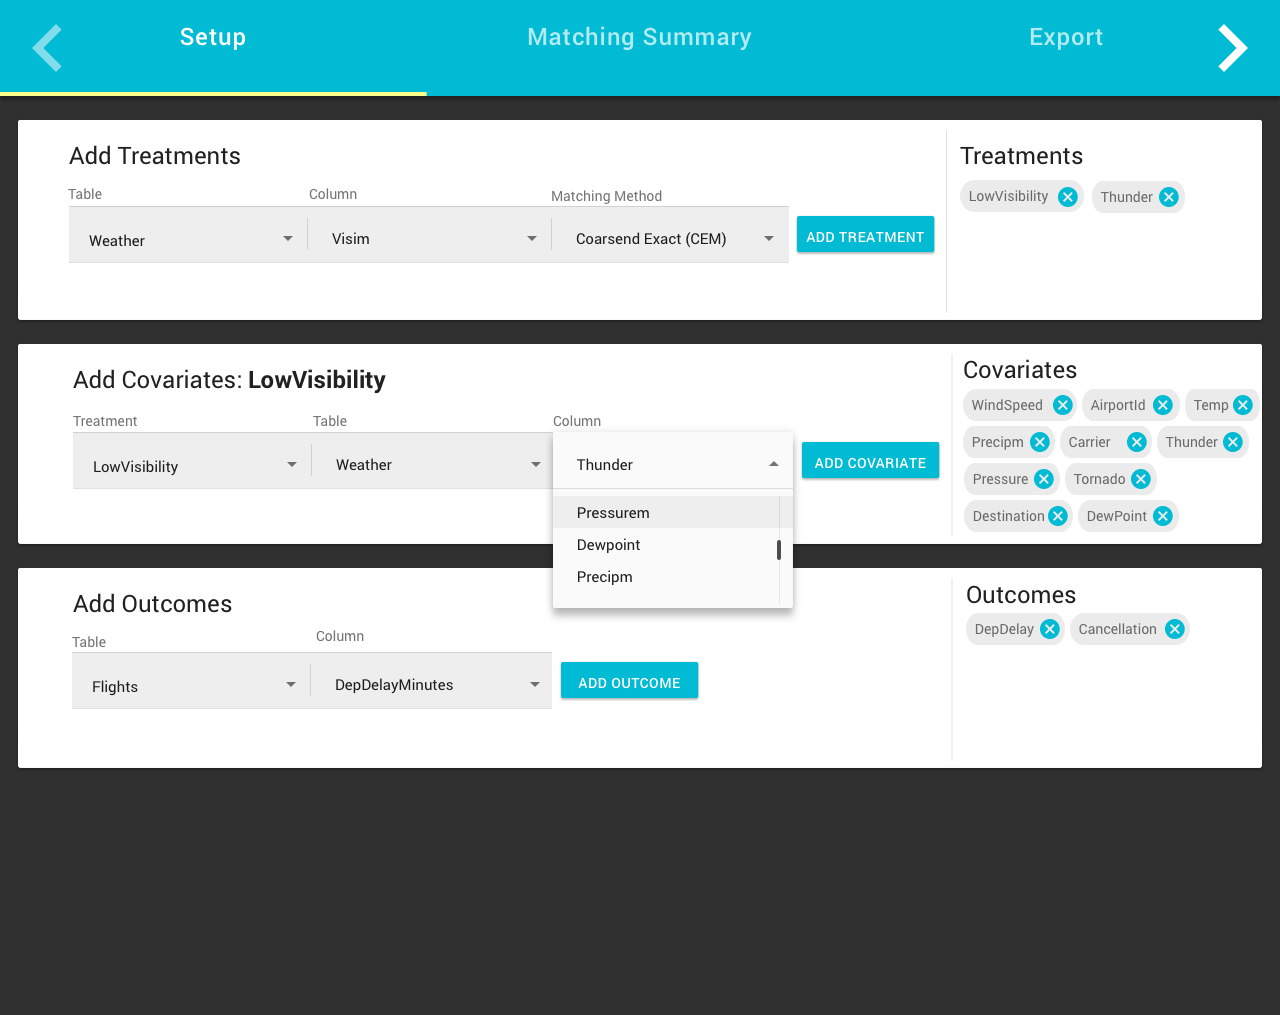
\includegraphics[scale=0.13]{Figures/Setup.png}
\label{sfig:testc}
\end{subfigure}\hfill
\begin{subfigure}{0.47\linewidth}
\centering
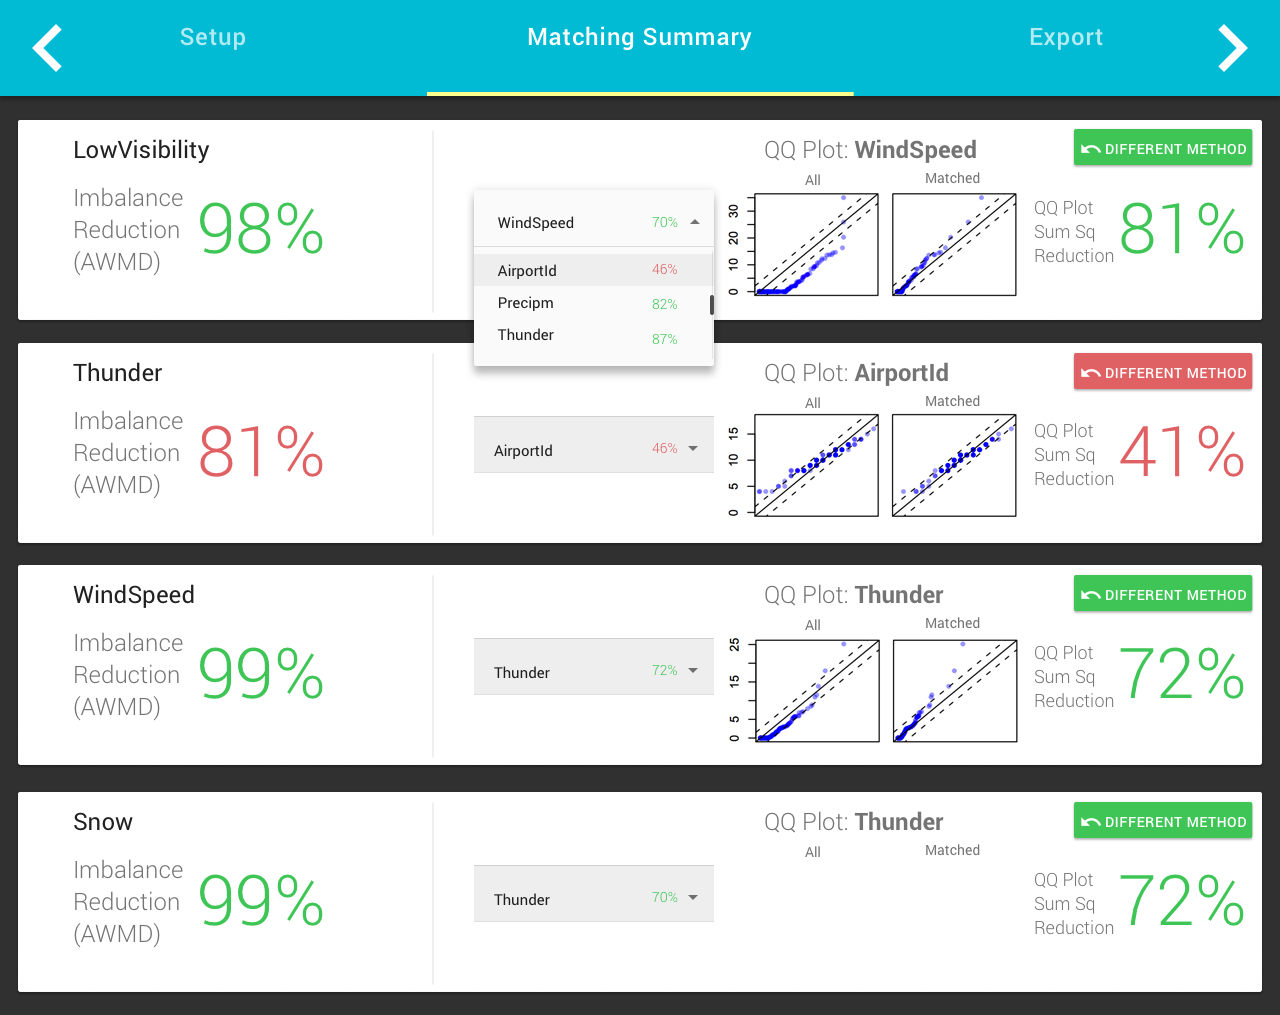
\includegraphics[scale=0.13]{Figures/Matching-Summary.png}
\label{sfig:testd}
\end{subfigure}\hfill
\caption{Demonstration Screenshot described in Section \ref{sec:dd}}
\label{fig:eteresult}
\end{figure*}






 \ignore{

 \begin{table*}[!htb] \scriptsize
    \begin{subtable}{.5\linewidth}
      \centering

       \begin{tabular}[t]{|l|l|}
  \hline
  % after \\: \hline or \cline{col1-col2} \cline{col3-col4} ...
  \bf{Attribute}   & \bf{Description}  \\  \hline
  FlightDate & Flight date   \\ \hline
  UniqueCarrier	& Unique carrier code   \\ \hline
  OriginAirportID & 	Origin airport ID  \\ \hline
  CRSDepTime & Scheduled departure time  \\ \hline
  DepTime & Actual departure time \\ \hline
    & difference in minutes between   \\
  DepDelayMinutes & scheduled and actual departure \\
   & time. Early departures set to 0  \\ \hline
  LateAircraftDelay & Late aircraft delay, in minutes  \\ \hline
  SecurityDelay & Ssecurity delay, in minutes \\ \hline
  CarrierDelay & Carrier delay, in minutes  \\ \hline
  Cancelled & Binary indicator  \\
  \hline
\end{tabular}
     \caption{Flight dataset}
    \end{subtable}%
    \begin{subtable}{.5\linewidth}
      \centering


       \begin{tabular}[t]{|l|l|}
  \hline
  % after \\: \hline or \cline{col1-col2} \cline{col3-col4} ...
  \bf{Attribute}   & \bf{Description}  \\  \hline
  Code  & Airport ID    \\ \hline
  Date	& Date of a repost   \\ \hline
  Time        & Time of a report  \\ \hline
  Visim        & Visibility in km  \\ \hline
  Tempm & Temperature in C$^{\circ}$ \\ \hline
  Wspdm         & Wind speed kph \\ \hline
  \ignore{Precipm         & Humidity \% \\ \hline}
  Pressurem         & Pressure in mBar  \\ \hline
  Precipm         & Precipitation in mm  \\ \hline
  \ignore{Rain & Binary indictor    \\ \hline
  Snow & Binary indictor \\ \hline}
  Tornado & Binary indictor \\ \hline
  Thunder & Binary indictor \\ \hline
  Hum & Humidity \% \\ \hline
  Dewpoint & De point in  C$^{\circ}$ \\ \hline
\end{tabular}
        \caption{Weather dataset}
    \end{subtable}
 \vspace{-0.1cm}   \caption{\bf{List of attributes from the flight(a) and weather(b)  datasets that are relevant to our analysis.}}
\label{tab:attlist}
\end{table*}
 }
 \ignore{
 The analysis will be conducted on
 {\em flight data (105M eateries)}-collected by the US Department of Transportation (U.S. DOT)- and  {\em weather dataset} (10M eateries)-gathered using the weather underground
API. }

 \ignore{
 The {\em flight dataset} we use was collected by the US Department of Transportation (U.S. DOT) \cite{flightdata}. It contains
records of more than 90\% of US domestic flights of major airlines
from 1988 to the present. The {\em weather dataset} was gathered using the weather underground
API \cite{Weatherdata}.  \ignore{Its attributes are also presented in Table
\ref{tab:attlist}. In addition, we pre-computed two other attributes
AiportTraffic and CarrierTraffic. The former is the total number of
flights occur in the origin airport of a flight one hour prior to the
flight departure time, the latter is the same quantity restricted to
the flights from the same carrier.  We managed to acquire and clean
35M weather observations between 2000 and 2015.} These datasets are
integrated by a spatio-temporal join.}



\ignore{

        \caption{Weather dataset}
    \end{subtable}
 \vspace{-0.1cm}   \caption{\bf{List of attributes from the flight(a) and weather(b)  datasets that are relevant to our analysis.}}
\label{tab:attlist}
\end{table}
}



\begin{figure}
  
\includegraphics[scale=0.25]{Figures/Matching-Flowchart.png}
\caption{Causal Analysis Workflow}
\label{fig:flowchart}
\vspace{-0.3cm}
\end{figure}






\ignore{
\begin{example} \em \delay (cont.) \ \em   Suppose we want to explore the effect of the low-pressure (treatment) on flight departure delays (outcome).  The direct comparison of
delay between flights that happen during low-pressure (treated groups) and opposite (control group) is misleading.  It is known that high pressure is generally associated with clear weather,    while low-pressure is associated with unsettled weather, e.g.,
    cloudy, rainy, or snowy weather\ignore{\cite{weba2,barometricpressureheadache:article}}. Thus, as shown in Figure \ref{fig:cv}, factors such as thunder, snow, visibility confound pressure and delay. Therefore, conducting any sort of predictive analysis identifies
    low-pressure as a predictor for flight delays.
  However, low-pressure does not have any causal impact on departure delay
    (low-pressure only requires longer takeoff distance) \cite{FAA08}. In this demonstration, by conducting a careful causal analysis using \GSQL, we show that low-pressure is only a correlated attribute with flight delays and has no significant causal impact on flight delay.

    \ignore{By performing a careful casual analysis
    \GSQL\ found that other attributes such as thunder, low-visibility, high-wind-speed and
    snow have the largest causal effect on flight delays (see Sec. \ref{sec:endtoend});
  this is confirmed by the results reported by the FAA.}
\end{example}
}

% They defined a very simple model, where we
% want to conclude \dan{Lise: what's your comment here?}  if one
% variable, called ``treatment'' causes one particular output variable,
% called ``effect'', and have developed a rich set of techniques for
% that purpose.  The end goal of their analysis is to establish the
% average causal-treatment effect.  More recently, in the AI literature
% Pearl~\cite{pearl2010introduction,PearlBook2000} has extended this
% simple model by introducing {\em causal networks}, and developing a
% logical framework for reasoning about causality.  Their aim is to
% enable complex inference in a network of causal associations.  While
% the ultimate goal is the same, to check whether a particular input
% causes a particular outcome, the methods deployed are different from
% those in statistics.

\vspace{-0.1cm}

\ignore{
This paper makes the following specific contributions: we describe a
suite of techniques for expressing the existing advanced methods for
causal inference from observational data in SQL that run at scale
within a database engine (Section \ref{sec:BasicTechniques}). Note
that we do not claim any contribution the existing methods; we
introduce several optimization techniques that significantly speedup
causal inference, both in the online and offline setting (Section
\ref{sec:OptimizationTechniques}); we validate our system
experimentally, using real data from the U.S. DOT and Weather
Underground \cite{flightdata,Weatherdata}
}

\ignore{
Roughly speaking, in order to draw a valid causal conclusion one needs to control for the
confounding influences that affect both the treatment and outcome. Popular methods for
performing this task in statistics and social science are {\em subclassification and matching} \cite{Rubin1983b,IacKinPor09,rosenbaum1984reducing}.
The key goal of matching is to prune data so that
the remaining data have better balance between the treated and control groups meaning that the empirical distributions of the confounding variables (a.k.a, covariates) in the groups are more similar.  Since there is no generic metric to compare
two distributions a rule of thumb is to evaluate different matching methods and balance measures  until a well-balance matched subset with
a reasonable size obtained \cite{IacKinPor09} (See Figure \ref{fig:flowchart}).
}



\ignore{
\begin{enumerate}
\item {\it Selecting a causal hypothesis:}
  the attendee selects a causal hypothesis to test by specifying a treatment (potential cause)
  and an outcome (potential effect) (cf, Example \ref{sfig:testaa}).
\item {\it Matching method:} The user select a matching method to
\item Enable attendees to drill into the details of how we generate these
results (i.e.\, the different steps of the pipeline).
\item Show what happens for different configurations of the Viska system:
e.g.\, different parameters to graph-generation algorithms, different bucketing
strategies, \ldots
\end{enumerate}
}



  \paragraph{\bf Causal Questions:} demonstration starts by creating a set of causal questions regarding the effect of different weather attributes on flight delay by
    \begin{enumerate}
      \item specifying a set of binary treatments, e.g., low-visibility, Snow, \ldots (potential causes)
      \item specifying an outcome of interest (potential effect) e.g., departure delay, cancelation, \ldots
      \item specifying a subset of data that is relevant to the analysis with e.g., flights at JFK airport
\end{enumerate}

 As shown in Figure \ref{fig:eteresult}, we use \GSQL\ to define the following treatments:
 LowVisibility (1 if Visim$<1$; 0 if Visim$>5$); \
Snow (1 iff Precipm$>0.3$ and Tempm$<0$); \ WindSpeed (1 if
Wspdm$>40$; 0 if Wspdm$<20$); \  Thunder \ Low-Pressure (1 if Pressurem$<009.14$; 0 if Pressurem$>1022.69$). We quantify the effect of each of these treatments on flight departure delay, DepDelay, at five US airport with high rate of weather-related delay namely,
 following airports: San Francisco (SFO) , John F. Kennedy (JFK), Newark Liberty (EWR), George Bush (IAH), and LaGuardia Airport (LGA).

 \paragraph{ \bf Computing ATE}: For each treatment, say Low-Pressure, \GSQL\ computes {\em average treatment effect (ATE)} as $$E[\text{Depdelay}|\text{Low-Pressure}=1] - E[\text{Depdelay}|\text{Low-Pressure}=0].$$
 ATE in computed by taking the difference between the empirical average of Depdelay where Low-Pressure is 1 and 0. It compares the outcome of the {\em treated group}, those subjects (flights) with treatment=1, and the {\em control group}, those with treatment=0.
 For example, for Low-Pressure we obtain that ATE is a relatively large number. This result suggests that this treatment impact departure delay. However, it is known that
  low-pressure does not have any causal impact on departure delay (low-pressure only requires longer takeoff distance) \cite{FAA08}.  Thus, we show that the direct comparison of an outcome between the  treated and control groups could be very misleading.

 \paragraph{\bf Confounding variables:} We demonstrate the issues with the naive computation of
  ATE. We show that the observed  effect of Low-pressure reflect the {\em  confounding influence} of other variables such as visibility, snow and Thunder.  In fact, low pressure is generally associated with unsettled weather conditions that are actually affect flight delay. For instance the average of visibility in the treated group is much less than
  the opposite group. Thus, the observed difference could be the effect of low viability. In general, in the presentence of confounding variable (a.k., covariates) treated and control groups are very different. Thus, comparing the outcome between the two groups are is not a fair comparison.


 \paragraph{\bf Adjusting for confounding variables:}
We show that in order to draw a valid causal conclusion one needs to adjust for the
confounding influences. The popular methods for
performing this task in statistics and social science are {\em subclassification and matching} \cite{Rubin1983b,IacKinPor09,rosenbaum1984reducing}.
The key goal of matching is to prune data so that
the remaining data ({\em matched data}) have better balance between the treated and control groups meaning that the empirical distributions of the confounding variables in the groups are more similar. Once the two groups become similar on every relevant aspect the comparison between them would be fair and meaningful. In this step of the demonstration we use \GSQL\ for performing the following steps:

     \begin{enumerate}
      \item For each treatment, we specify a set of covariates deemed to confound with the the DepDelay (Figure \ref{fig:eteresult}(a))
      \item We select a matching method supported by \GSQL\ and adjust its tuning parameters (Figure \ref{fig:eteresult}(b))
\end{enumerate}

\paragraph{\bf Checking Balance:}  In this step we check weather the matching method was successful to achieve its goal which was to improve balance by
    \begin{enumerate}
      \item comparing the distribution for each covariate between the treated and control groyp after matching. In particular, usees numerical summaries such as the mean Diff. (difference in means), and summaries based on quantile quantile plots and multivariate histograms to compare the empirical distributions of each covariate between the treated and control group in the matched data.

      \item We perform different matching methods with difference turning parameter to show how these techniques trade of balance and size of matched subset as exemplified in Figure \ref{fig:eteresult}(b).
       \end{enumerate}
      This goal of this step of the demonstration meant to illustrate the typical worlkflow of causal inference from observational data as depicted in picture \ref{fig:flowchart}.

     \paragraph{\bf Answer causal question:} In this step of the demonstration we answer the causal question created at the very fist step of the demonstration.

       \begin{enumerate}
       \item For each treatment we compute ATE on an associated matched subset of data.
      \item We evaluate the statistical significance of the obtained result by performing an statistical test, e.g., Chi-square, test on the matched data.
    \item We perform the above steps for each airport to find out the major weather related causes of delay.  
    \end{enumerate}

Finally, we show that the results are those of
FAA, which reported the following major weather-related
causes of flight delay at the airports under the study:
snowstorms,thunderstorm and wind at EWR; thunderstorm and fog at IAH;
snowstorms and visibility at JFK; snowstorms at LGA; fog and low
clouds at SFO;




